\silentchapter{Anexe}
%% Nu se pot face referinte pe silentchapter => nu are sens sa pun label
% \label{cap:anexe}

Această secțiune cuprinde, pe de o parte, diagramele de proiectare ale sistemului (cazurile de utilizare, diagrama de clase a tiparelor arhitecturale și diagrama relațională a bazei de date), iar pe de altă parte, fragmente reprezentative din codul sursă dezvoltat în cadrul lucrării, prea extinse pentru a fi incluse în corpul acesteia, dar relevante pentru înțelegerea componentelor centrale ale soluției: task-ul de provizionare asincronă, mecanismul de evenimente de domeniu care realizează decuplarea și suita de teste end-to-end.

\newpage
\section{Diagrama cazurilor de utilizare}
\label{anexa:usecase}

Figura~\ref{fig:usecase} prezintă diagrama cazurilor de utilizare a platformei, cu cei trei actori (membru, proprietar, administrator) și relația de specializare dintre ei, referită în Secțiunea~\ref{sec:cap3_cerinte}.

\begin{figure}[H]
    \centering
    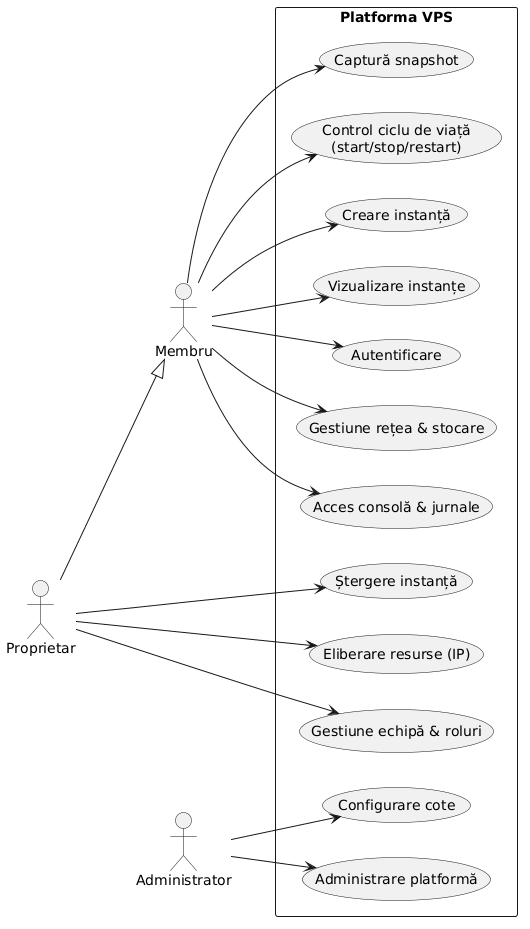
\includegraphics[height=0.8\textheight,keepaspectratio]{continut/capitol3/figuri/usecase.png}
    \caption{Diagrama cazurilor de utilizare a platformei.}
    \label{fig:usecase}
\end{figure}

\newpage
\section{Diagrama de clase a tiparelor de proiectare}
\label{anexa:class}

Figura~\ref{fig:class_diagram} prezintă diagrama de clase a tiparelor de proiectare din nivelul backend (Repository, Unit of Work și Domain Events), referită în Secțiunea~\ref{sec:cap3_tipare}.

\begin{figure}[H]
    \centering
    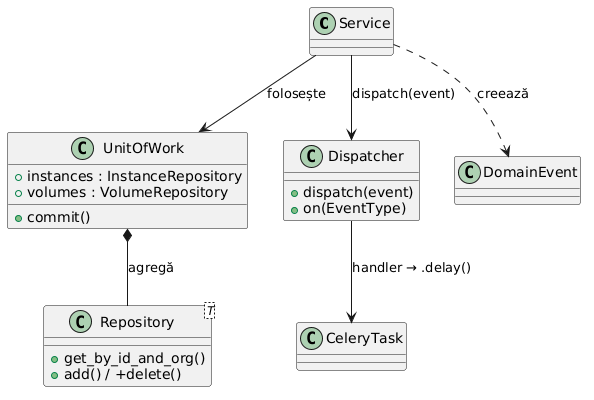
\includegraphics[width=0.9\textwidth]{continut/capitol3/figuri/class_diagram.png}
    \caption{Diagrama de clase a tiparelor de proiectare din nivelul backend.}
    \label{fig:class_diagram}
\end{figure}

\newpage
\section{Diagrama relațională a bazei de date}
\label{anexa:er}

Figura~\ref{fig:er_diagram} prezintă diagrama Entity-Relationship a entităților din baza de date MariaDB, referită în Secțiunea~\ref{sec:cap3_baza_date}.

\begin{figure}[H]
    \centering
    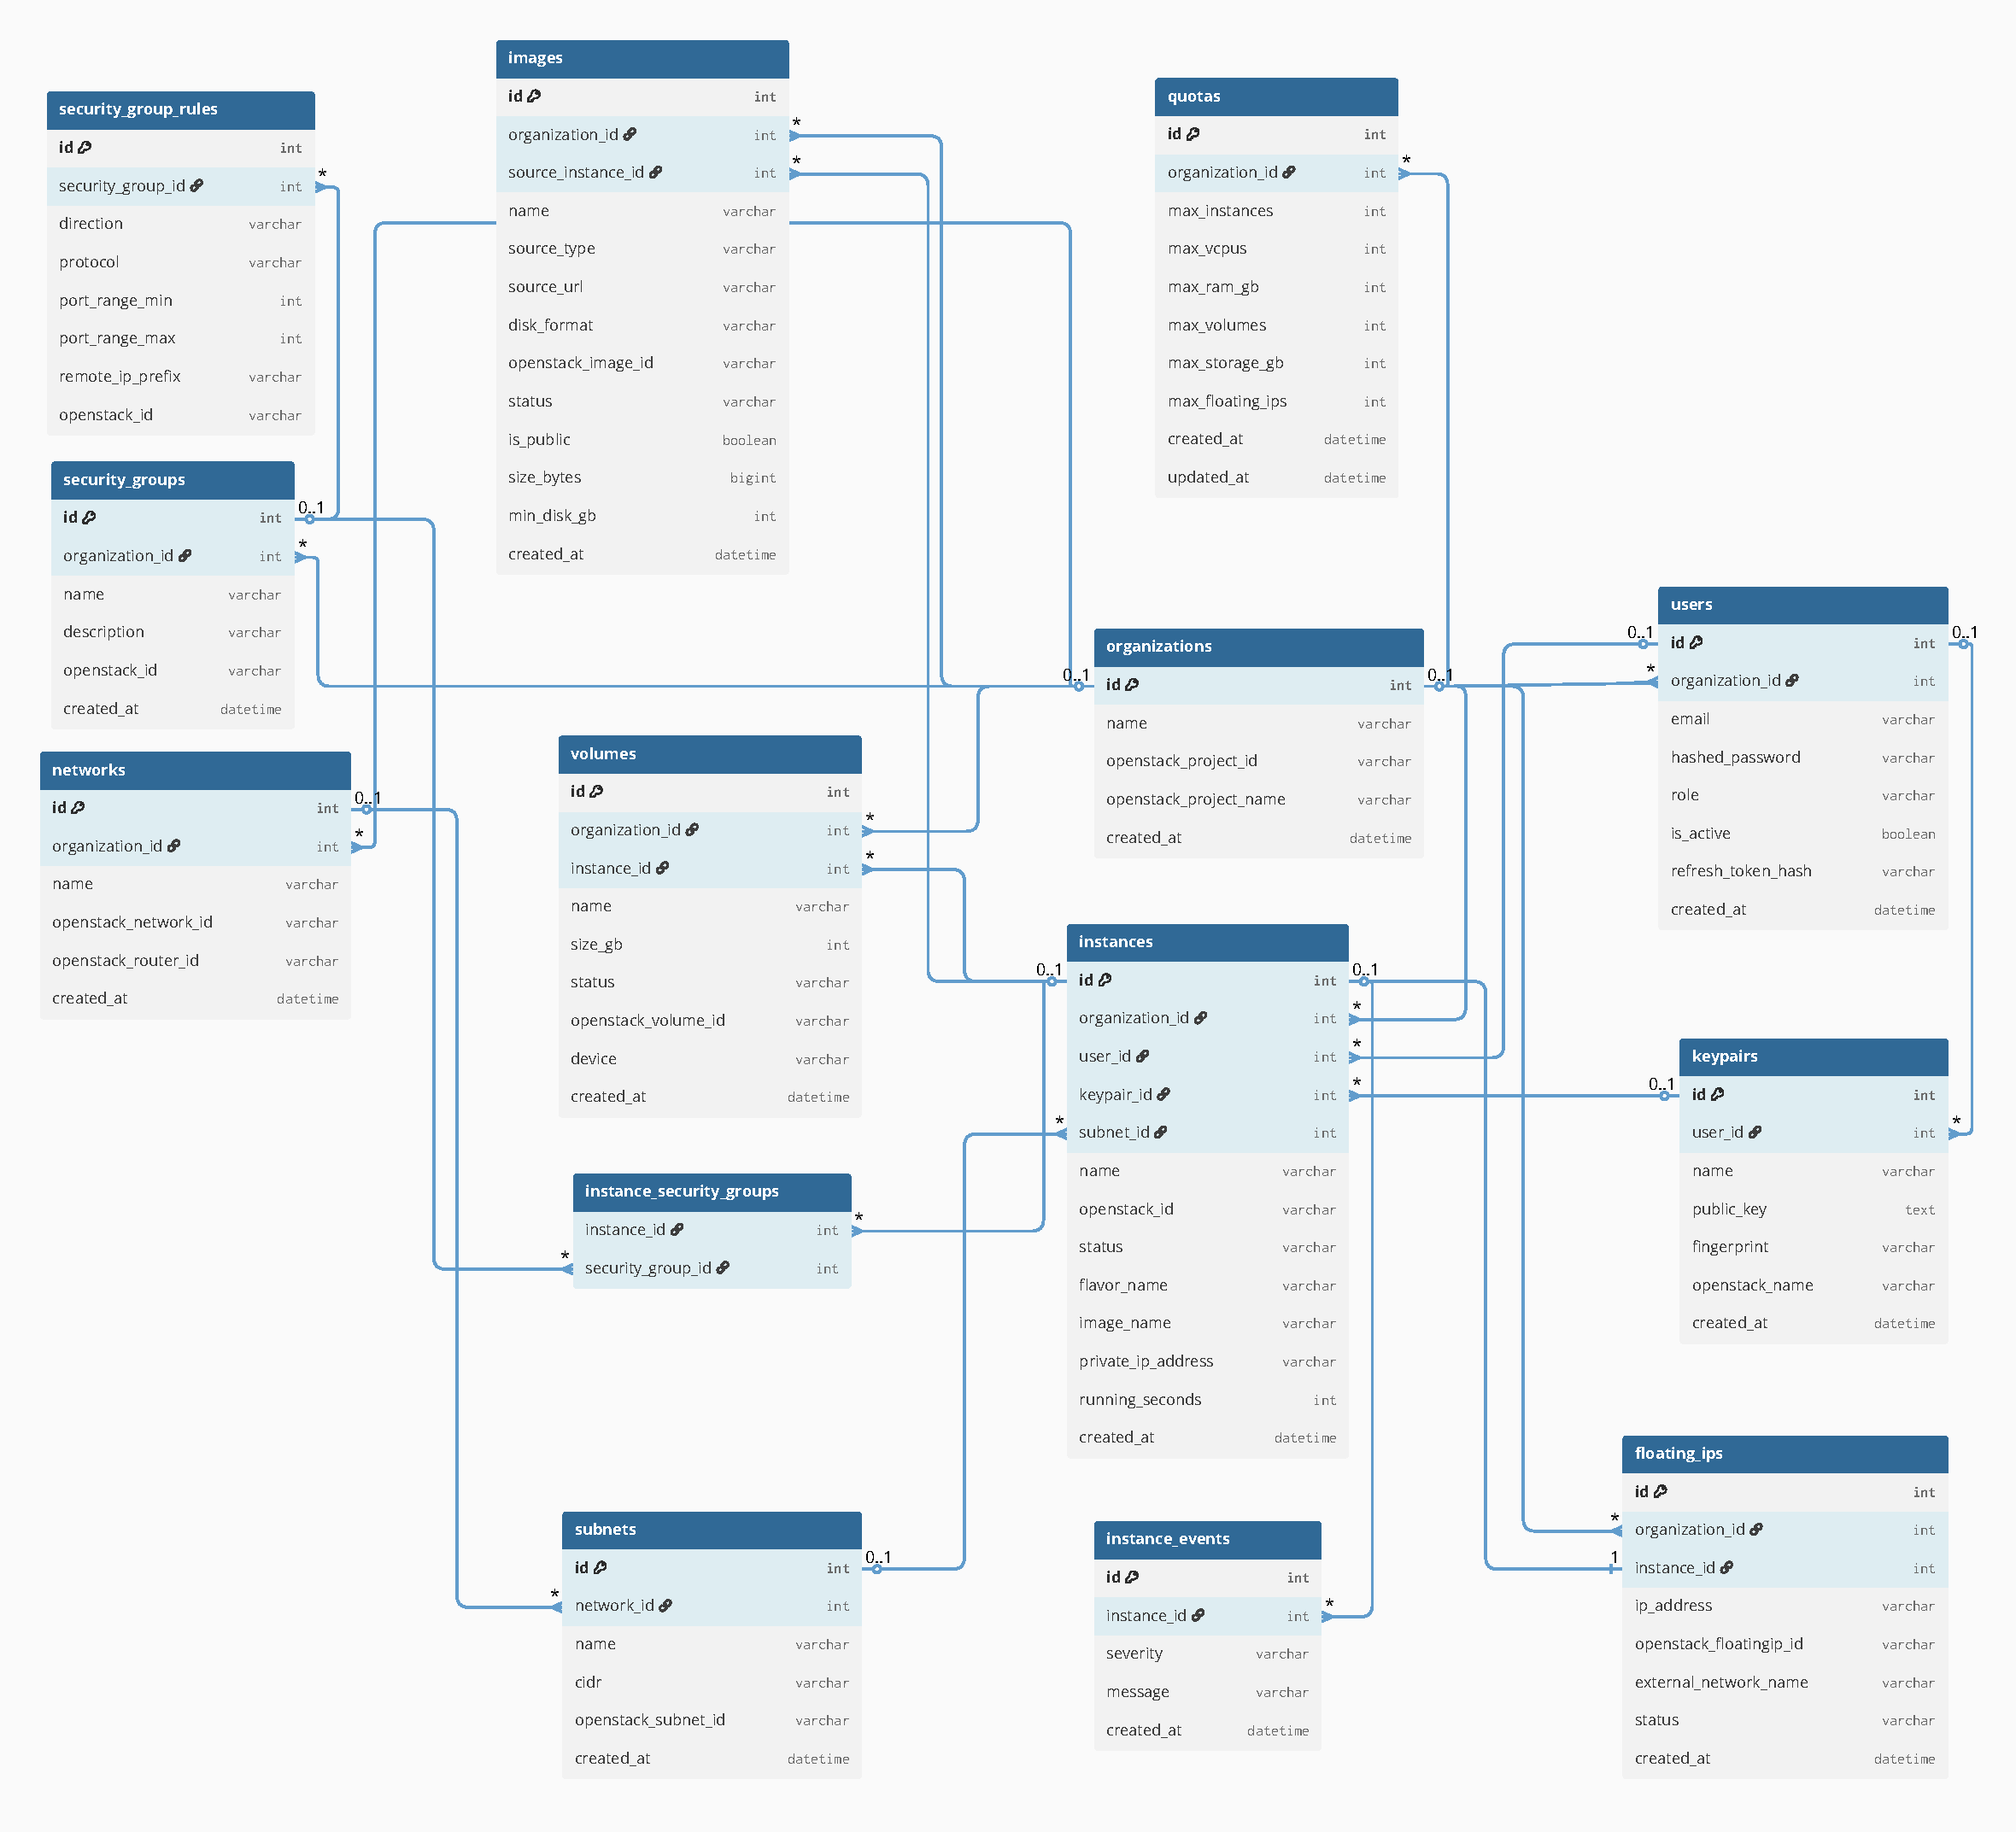
\includegraphics[width=\textwidth]{continut/capitol3/figuri/er_diagram.pdf}
    \caption{Diagrama relațională (ER) a entităților din baza de date MariaDB.}
    \label{fig:er_diagram}
\end{figure}

\newpage
\section{Task-ul de provizionare asincronă a unei instanțe}
\label{anexa:provision}

Listing-ul~\ref{code:provision} prezintă task-ul Celery \texttt{provision\_instance}, care concentrează întreaga interacțiune cu infrastructura OpenStack la crearea unei mașini virtuale: rezolvarea imaginii, a pachetului hardware și a cheii, crearea serverului prin Nova, așteptarea tranziției în starea \texttt{ACTIVE}, actualizarea bazei de date, alocarea opțională a unei adrese IP publice și atașarea volumelor, precum și tratarea erorilor cu reîncercare automată.

\begin{lstlisting}[language=Python, basicstyle=\ttfamily\scriptsize, breaklines=true, frame=single, numbers=left, numberstyle=\tiny, showstringspaces=false, caption={Task-ul Celery \texttt{provision\_instance} (\texttt{tasks/vm\_tasks.py}).}, label={code:provision}]
@celery_app.task(bind=True, max_retries=3)
def provision_instance(
    self,
    instance_id: int,
    name: str,
    image_name: str,
    flavor_name: str,
    keypair_openstack_name: str,
    subnet_openstack_id: str,
    security_group_openstack_ids: list[str],
    root_disk_gb: int = 0,
    data_volume_size_gb: int = 0,
    attach_volume_ids: list[int] | None = None,
    user_data: str = "",
    assign_floating_ip: bool = True,
):
    print(f"[Task {self.request.id}] Provisioning instance '{name}' (db_id={instance_id})")
    try:
        conn = _os_connect()

        image = conn.compute.find_image(image_name)
        flavor = conn.compute.find_flavor(flavor_name)
        keypair = conn.compute.find_keypair(keypair_openstack_name)

        if not all([image, flavor, keypair]):
            raise Exception(
                f"OpenStack resource not found - image={image}, flavor={flavor}, keypair={keypair}"
            )

        # Resolve the tenant network from the subnet before creating the server
        subnet_obj = conn.network.get_subnet(subnet_openstack_id)
        network_id = subnet_obj.network_id

        server_kwargs = dict(
            name=name,
            flavor_id=flavor.id,
            networks=[{"uuid": network_id}],
            key_name=keypair.name,
            security_groups=[{"name": sg_id} for sg_id in security_group_openstack_ids],
        )
        if root_disk_gb and root_disk_gb > 0:
            # boot from a fresh Cinder volume created from the image (custom root disk);
            # delete_on_termination ties the boot volume to the instance lifecycle
            server_kwargs["block_device_mapping_v2"] = [{
                "boot_index": 0,
                "uuid": image.id,
                "source_type": "image",
                "destination_type": "volume",
                "volume_size": root_disk_gb,
                "delete_on_termination": True,
            }]
        else:
            # default: ephemeral root disk sized by the flavor
            server_kwargs["image_id"] = image.id

        if user_data:
            # nova expects user_data base64-encoded; cloud-init runs it on first boot
            server_kwargs["user_data"] = base64.b64encode(
                user_data.encode("utf-8")).decode("ascii")

        server = conn.compute.create_server(**server_kwargs)

        print(f"[Task {self.request.id}] Waiting for server to become ACTIVE...")
        server = conn.compute.wait_for_server(server)

        # Extract the private IP from the tenant network
        private_ip = None
        for net_name, addresses in server.addresses.items():
            if addresses:
                private_ip = addresses[0]["addr"]
                break

        # Update the instance record with the OpenStack info
        with SessionLocal() as db:
            instance = db.query(Instance).filter(Instance.id == instance_id).first()
            if instance:
                instance.openstack_id = server.id
                instance.private_ip_address = private_ip
                instance.status = "ACTIVE"
                db.commit()

        _log_event(instance_id, "info", f"Instance is active (private IP {private_ip})")

        # Allocate and associate a floating IP from the external pool,
        # only when the user opted in on the create form (default on)
        if assign_floating_ip:
            _allocate_floating_ip(conn, instance_id, server.id, network_id)

        # Create/attach any requested block-storage volumes (best-effort)
        try:
            _attach_instance_volumes(
                conn, instance_id, server.id, data_volume_size_gb, attach_volume_ids or [])
        except Exception as vol_exc:
            _log_event(instance_id, "warning", f"Volume setup failed: {vol_exc}")

        return {"status": "success", "instance_id": instance_id, "private_ip": private_ip}

    except Exception as exc:
        print(f"[Task {self.request.id}] ERROR: {exc}")
        with SessionLocal() as db:
            instance = db.query(Instance).filter(Instance.id == instance_id).first()
            if instance:
                instance.status = "ERROR"
                db.commit()
        _log_event(instance_id, "error", f"Provisioning failed: {exc}")
        raise self.retry(exc=exc, countdown=15)
\end{lstlisting}

\newpage
\section{Mecanismul de evenimente de domeniu}
\label{anexa:evenimente}

Decuplarea serviciilor de procesarea asincronă se realizează printr-un dispecer minimal (Listing-ul~\ref{code:dispatcher}): gestionarii se înregistrează pentru un tip de eveniment prin decoratorul \texttt{@on}, iar funcția \texttt{dispatch} rutează fiecare eveniment către gestionarii săi.

\begin{lstlisting}[language=Python, basicstyle=\ttfamily\scriptsize, breaklines=true, frame=single, numbers=left, numberstyle=\tiny, showstringspaces=false, caption={Dispecerul de evenimente (\texttt{domain/dispatcher.py}).}, label={code:dispatcher}]
from collections import defaultdict
from typing import Callable
from domain.events import DomainEvent

# Registry: event type -> list of synchronous handler callables
_handlers: dict[type[DomainEvent], list[Callable[[DomainEvent], None]]] = defaultdict(list)


def on(event_type: type[DomainEvent]) -> Callable:
    """Decorator to register a handler for a specific event type."""
    def decorator(fn: Callable[[DomainEvent], None]) -> Callable:
        _handlers[event_type].append(fn)
        return fn
    return decorator


def dispatch(event: DomainEvent) -> None:
    """Call every registered handler for this event type in registration order."""
    for handler in _handlers[type(event)]:
        handler(event)
\end{lstlisting}

Evenimentele sunt simple obiecte de date (Listing-ul~\ref{code:event}), iar gestionarul corespunzător, înregistrat în stratul Celery, nu face decât să declanșeze task-ul asincron, transferând datele evenimentului. 

\begin{lstlisting}[language=Python, basicstyle=\ttfamily\scriptsize, breaklines=true, frame=single, numbers=left, numberstyle=\tiny, showstringspaces=false, caption={Definirea unui eveniment de domeniu și gestionarul asociat.}, label={code:event}]
# domain/events.py
@dataclass
class DomainEvent:
    event_id: str = field(default_factory=lambda: str(uuid4()))
    occurred_at: datetime = field(default_factory=lambda: datetime.now(timezone.utc))


@dataclass
class InstanceProvisioningStarted(DomainEvent):
    """Raised by the service layer after the DB record is created with status=BUILD.
    Celery picks this up and performs the actual OpenStack work."""
    instance_id: int = 0
    name: str = ""
    image_name: str = ""
    flavor_name: str = ""
    keypair_openstack_name: str = ""
    subnet_openstack_id: str = ""
    security_group_openstack_ids: list[str] = field(default_factory=list)
    assign_floating_ip: bool = True


# tasks/vm_tasks.py
@on(InstanceProvisioningStarted)
def handle_provisioning_started(event: InstanceProvisioningStarted) -> None:
    provision_instance.delay(
        instance_id=event.instance_id,
        name=event.name,
        image_name=event.image_name,
        flavor_name=event.flavor_name,
        keypair_openstack_name=event.keypair_openstack_name,
        subnet_openstack_id=event.subnet_openstack_id,
        security_group_openstack_ids=event.security_group_openstack_ids,
        assign_floating_ip=event.assign_floating_ip,
    )
\end{lstlisting}

\newpage
\section{Suita de teste end-to-end automate}
\label{anexa:teste}

Listing-ul~\ref{code:teste} prezintă nucleul suitei de teste automate descrise în Capitolul~\ref{cap:cap4}: funcția ajutătoare de interogare periodică (\textit{polling}), care gestionează caracterul asincron al provizionării, și testele care validează ciclul de viață al unei instanțe pe infrastructura OpenStack reală --- lansarea și tranziția în starea \texttt{ACTIVE}, ciclul de oprire/pornire și ștergerea. Fiecare test acționează asupra stivei vii prin HTTP, exact ca un client. Raportul de execuție generat la rularea suitei (\texttt{pytest -m e2e}) este prezentat în Figura~\ref{fig:cap4_pytest}, confirmând trecerea tuturor scenariilor automate.

\begin{figure}[H]
    \centering
    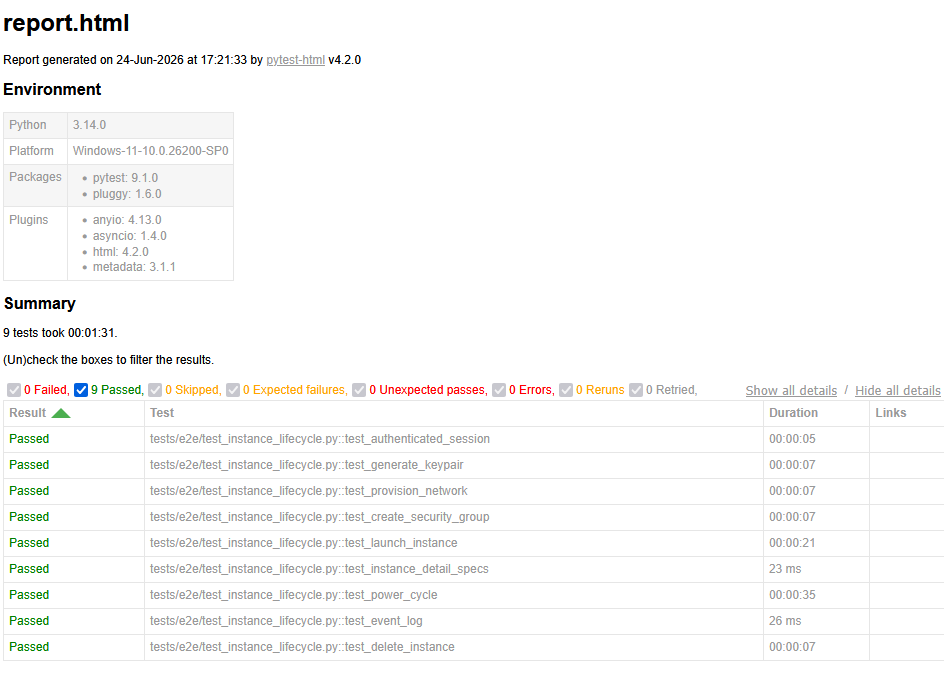
\includegraphics[width=\textwidth]{continut/capitol4/figuri/pytest-html.png}
    \caption{Raportul de execuție al suitei de teste end-to-end.}
    \label{fig:cap4_pytest}
\end{figure}

\begin{lstlisting}[language=Python, basicstyle=\ttfamily\scriptsize, breaklines=true, frame=single, numbers=left, numberstyle=\tiny, showstringspaces=false, caption={Nucleul suitei de teste E2E (\texttt{tests/e2e/}).}, label={code:teste}]
# tests/e2e/conftest.py
def poll(fetch, ready, timeout, interval, what):
    """Call fetch every interval seconds until ready(result) is true.
    Returns the satisfying result, or raises AssertionError after timeout."""
    deadline = time.monotonic() + timeout
    last = None
    while time.monotonic() < deadline:
        last = fetch()
        if ready(last):
            return last
        time.sleep(interval)
    raise AssertionError(f"Timed out after {timeout}s waiting for {what}")


# tests/e2e/test_instance_lifecycle.py
def test_launch_instance(client, ctx):
    """CF5 - the API accepts the request immediately (status BUILD), then the
    background worker provisions it on OpenStack until it reaches ACTIVE."""
    payload = {
        "name": "e2e-vm",
        "flavor_name": FLAVOR,
        "image_name": IMAGE,
        "keypair_id": ctx["keypair_id"],
        "subnet_id": ctx["subnet_id"],
        "security_group_ids": [ctx["sg_id"]],
        "assign_floating_ip": ASSIGN_FIP,
    }

    r = client.post("/instances/", json=payload)
    assert r.status_code == 201, r.text

    instance = r.json()[0]
    assert instance["status"] == "BUILD"   # accepted immediately (non-blocking)
    ctx["instance_id"] = instance["id"]

    detail = poll(
        lambda: client.get(f"/instances/{ctx['instance_id']}").json(),
        lambda d: d["status"] not in _TRANSIENT,
        PROVISION_TIMEOUT, POLL_INTERVAL, "instance to leave a transient state",
    )

    if detail["status"] != "ACTIVE":
        events = client.get(f"/instances/{ctx['instance_id']}/events").json()
        errors = [e["message"] for e in events if e["severity"] == "error"]
        reason = errors[-1] if errors else "(no error event)"
        pytest.fail(f"instance settled in {detail['status']} instead of ACTIVE - {reason}")
    assert detail["private_ip_address"], "ACTIVE instance has no private IP"


def test_power_cycle(client, ctx):
    """CF6 - stop then start the instance, asserting the expected terminal states."""
    iid = ctx["instance_id"]

    assert client.post(f"/instances/{iid}/stop").status_code == 200
    d = poll(
        lambda: client.get(f"/instances/{iid}").json(),
        lambda d: d["status"] not in _TRANSIENT,
        PROVISION_TIMEOUT, POLL_INTERVAL, "instance to stop",
    )
    assert d["status"] == "SHUTOFF"

    assert client.post(f"/instances/{iid}/start").status_code == 200
    d = poll(
        lambda: client.get(f"/instances/{iid}").json(),
        lambda d: d["status"] not in _TRANSIENT,
        PROVISION_TIMEOUT, POLL_INTERVAL, "instance to start",
    )
    assert d["status"] == "ACTIVE"


def test_delete_instance(client, ctx):
    """CF6 - delete the instance and confirm it disappears (resources released)."""
    iid = ctx["instance_id"]
    assert client.delete(f"/instances/{iid}").status_code == 200

    poll(
        lambda: client.get(f"/instances/{iid}").status_code,
        lambda code: code == 404,
        PROVISION_TIMEOUT, POLL_INTERVAL, "instance to be fully deleted",
    )
\end{lstlisting}
